% Slides for talk on hydrogen fuel cells
% given in the department on October 27, 2003.
% 
% The original slides were in Prosper.  This file contains the
% translation of the original slides to Beamer.
% 
% Rouben Rostamian <rostamian@umbc.edu>
% August 31, 2004

\documentclass[10pt]{beamer}
\usetheme{umbc4}
\useinnertheme{umbcboxes}
\setbeamercolor{umbcboxes}{bg=violet!12,fg=black}

\usepackage{rotating} % for defining \schwa
\newcommand{\schwa}{\raisebox{1ex}{\begin{turn}{180}e\end{turn}}}

\newcommand{\arcsinh}{\mathop\mathrm{arcsinh}\nolimits}
\newcommand{\arccosh}{\mathop\mathrm{arccosh}\nolimits}
\newcommand{\Pu}{P_{\mathrm{amb}}}

\title{Openyoudao}
% \subtitle{Modeling and Computations}
% \author[R. Rostamian]{Rouben Rostamian}
\institute[UMBC]{
  It is a YouDao client for linux \\
  Author: justzx2011@gmail.com  @justzx \\
          lvzongting@gmail.com  @lvzongting \\
   Powered by xdlinux.info  西电开源社区
}
\date{September 17, 2012}
\begin{document}

%----------- titlepage ----------------------------------------------%
\begin{frame}[plain]
  \titlepage
\end{frame}

%----------- slide --------------------------------------------------%
\begin{frame}
  \frametitle{History 2012--04--16 A boring Day!!!}

\begin{center} 
  
\includegraphics[width=0.4\textwidth]{pic1.jpg}
\end{center}
\medskip
\quad
\qquad

I am linuxer, Reading paper just so boring, I can't bear it any more!!!
\end{frame}

%----------- slide --------------------------------------------------%
\begin{frame}
  \frametitle{Some one can help me?}

\begin{center} 
  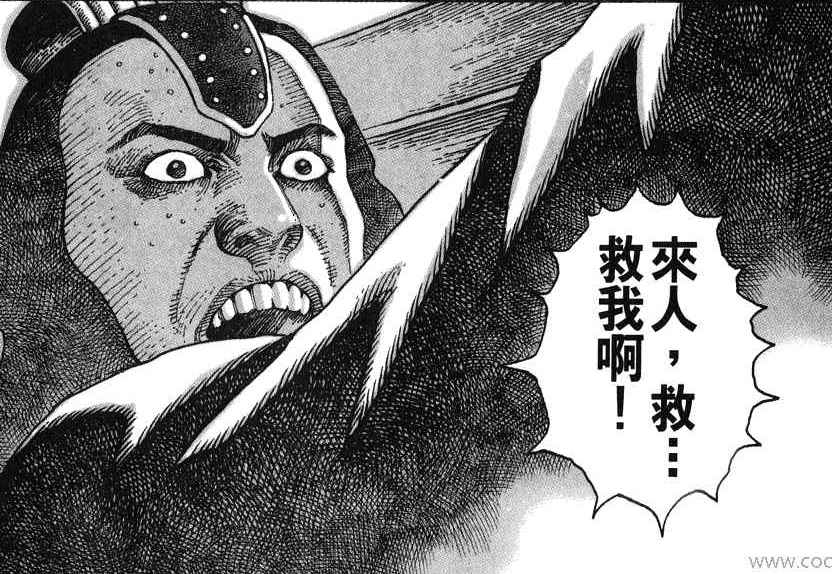
\includegraphics[width=0.6\textwidth]{help.jpg}
\end{center}

\end{frame}

%----------- slide --------------------------------------------------%
\begin{frame}
  \frametitle{Fuck! Writing one by myself}
 
\begin{center} 
  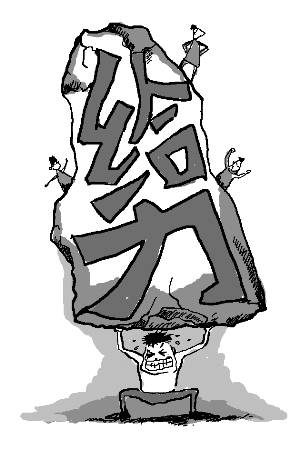
\includegraphics[width=0.4\textwidth]{geili.jpg}
  
\end{center}

\end{frame}

%----------- slide --------------------------------------------------%
\begin{frame}
  \frametitle{History 2012--05--28 A new life born}

\begin{center} 
  
\includegraphics[width=0.6\textwidth]{newlife.jpg}
 
\end{center}

\end{frame}

%----------- slide --------------------------------------------------%
\begin{frame}
  \frametitle{A sunny boy with Simple Profile}
\begin{center} 
  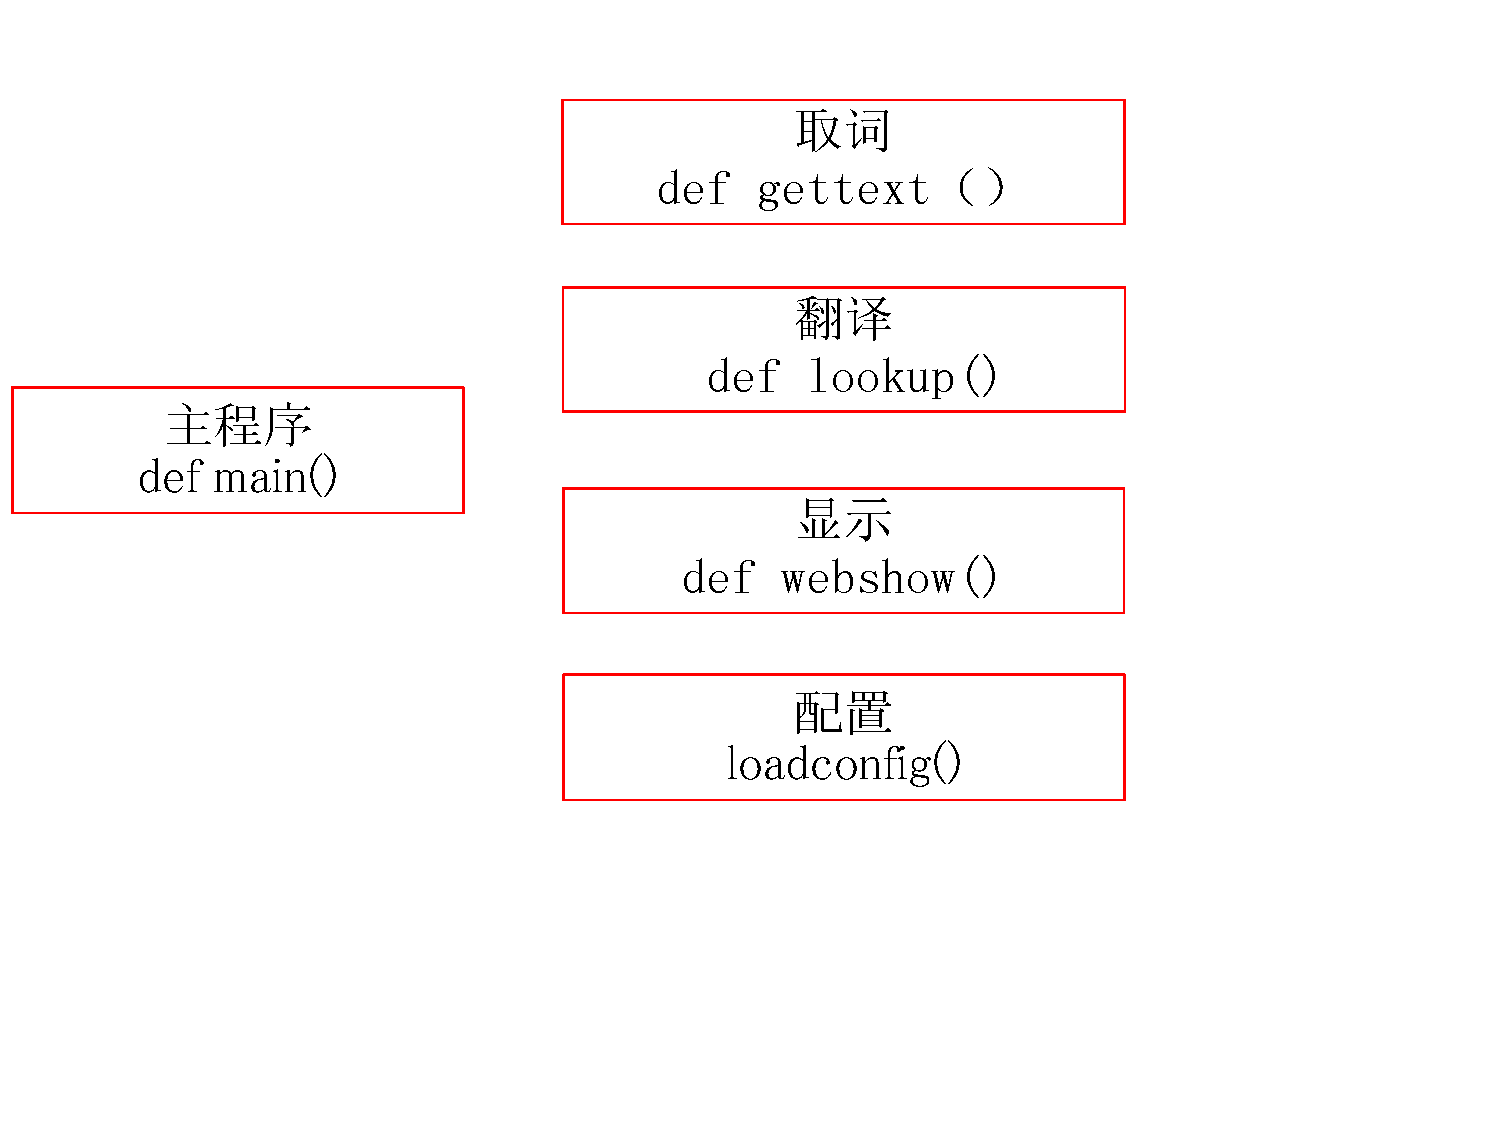
\includegraphics[width=1.1\textwidth]{construct.pdf}

\end{center}

\end{frame}

%----------- slide --------------------------------------------------%
\begin{frame}
  \frametitle{Gettext}
  pipe = os.popen("xclip -o") \\
  text = pipe.readline() \\
  cachedir = userdir + "/.openyoudao"\\
  historydir = cachedir + "/cache/history.cache"\\
  fin,fout = popen2.popen2("tee -a history.txt")\\


\end{frame}

%----------- slide --------------------------------------------------%
\begin{frame}
  \frametitle{Lookup}
  
cmd = "tail -f history.txt"\\
myfile=os.popen(cmd)\\
text=myfile.readline()\\
url= gl.baseurl + text\\


\end{frame}

%----------- slide --------------------------------------------------%
\begin{frame}
  \frametitle{webshow}

gl.homeurl="file://" + gl.resultdir\\
window.load(gl.homeurl)
window.show()  
\end{frame}

%----------- slide --------------------------------------------------%
\begin{frame}
  \frametitle{loadconfig}

cmdswitch = "inotifywait  -m " + gl.datadir\\
switch=os.popen(cmdswitch)\\
\end{frame}

%----------- slide --------------------------------------------------%
\begin{frame}
  \frametitle{To Do Next...}

OCR\\
terminal\\
Offline translate\\
icloud
\end{frame}

%----------- slide --------------------------------------------------%
\begin{frame}
  \frametitle{Release}

AUR\\
PPA\\
RPM
\end{frame}

%----------- slide --------------------------------------------------%
\begin{frame}
  \frametitle{Join Us}

http://openyoudao.org/\\
https://github.com/justzx2011/openyoudao\\
justzx2011@gmail.com  @justzx\\
lvzongting@gmail.com  @lvzongting\\

\end{frame}

%----------- slide --------------------------------------------------%
\begin{frame}
  \frametitle{Thanks}
Thanks!
\end{frame}

%----------- slide 

\end{document}
